\documentclass{article}
\usepackage[utf8]{inputenc}
\usepackage[spanish]{babel}
\usepackage{listings}
\usepackage[document]{ragged2e}
\usepackage{graphicx}
\usepackage{url}

\usepackage{color}


\definecolor{mygreen}{rgb}{0,0.6,0}
\definecolor{mygray}{rgb}{0.5,0.5,0.5}
\definecolor{mymauve}{rgb}{0.58,0,0.82}
\lstset{ 
  backgroundcolor=\color{white},   % choose the background color; you must add \usepackage{color} or \usepackage{xcolor}; should come as last argument
  basicstyle=\footnotesize,        % the size of the fonts that are used for the code
  breakatwhitespace=false,         % sets if automatic breaks should only happen at whitespace
  breaklines=true,                 % sets automatic line breaking
  captionpos=b,                    % sets the caption-position to bottom
  commentstyle=\color{mygreen},    % comment style
  deletekeywords={...},            % if you want to delete keywords from the given language
  escapeinside={\%}{)},          % if you want to add LaTeX within your code
  extendedchars=true,              % lets you use non-ASCII characters; for 8-bits encodings only, does not work with UTF-8
  firstnumber=1,                % start line enumeration with line 1000
  frame=single,	                   % adds a frame around the code
  keepspaces=true,                 % keeps spaces in text, useful for keeping indentation of code (possibly needs columns=flexible)
  keywordstyle=\color{blue},       % keyword style
  language=Octave,                 % the language of the code
  morekeywords={*,...},            % if you want to add more keywords to the set
  numbers=left,                    % where to put the line-numbers; possible values are (none, left, right)
  numbersep=5pt,                   % how far the line-numbers are from the code
  numberstyle=\tiny\color{mygray}, % the style that is used for the line-numbers
  rulecolor=\color{black},         % if not set, the frame-color may be changed on line-breaks within not-black text (e.g. comments (green here))
  showspaces=false,                % show spaces everywhere adding particular underscores; it overrides 'showstringspaces'
  showstringspaces=false,          % underline spaces within strings only
  showtabs=false,                  % show tabs within strings adding particular underscores
  stepnumber=1,                    % the step between two line-numbers. If it's 1, each line will be numbered
  stringstyle=\color{mymauve},     % string literal style
  tabsize=2,	                   % sets default tabsize to 2 spaces
  title=\lstname                  % show the filename of files included with \lstinputlisting; also try caption instead of title
}
\title{Tarea 2}

\author{5271}
\date{\today}

\begin{document}
\maketitle
\section{Introducción}
Cuando una información se manifiesta mediante objetos y sus relaciones, visualizarla puede ser el primer paso para resolver problemas de diversa índole. 
La modelación y teoría de grafos constituyen la forma más común de modelar información relacional, y su visualización una forma de representar la información \cite {tesis}.\linebreak

Sin embargo el modelado y acomodo de un grafo que refleje situaciones de la vida real resulta complejo, es por ello que se han desarrollado algoritmos dedicados a perfeccionar el trazado de los mismos según el tipo problema y grafo que representen, llamados algoritmos de diseño o \textit{layout}.\linebreak

Los algoritmos de diseño son los que devuelven una lista de posiciones para los nodos según diversos parámetros definidos para cada algoritmo, buscando cumplir con ciertos criterios estéticos como son: minimizar cruces entre aristas, maximizar el ángulo entre aristas adyacentes, maximizar el ángulo entre aristas que se cruzan, mostrar simetría, distribución uniforme de los vértices y longitud uniforme de aristas \cite {tesis}.\linebreak

Entre los algoritmos de diseño destacan los siguientes:

\begin{itemize}
 \item\textit{Bipartite layout} (posiciona los nodos en dos líneas rectas, es decir que divide el conjunto de nodos en dos subconjuntos $ X $ e $ Y $ donde no existe adyacencia entre los elementos de un mismo subconjunto)  \cite{networkx}.  
 \item\textit{Circular layout} (ubica los nodos en forma circular) \cite{networkx}.
	\item\textit{Kamada kawai layout} (posiciona los nodos utilizando la función de costo de longitud de camino Kamada-Kawai) \cite{networkx}.
	\item\textit{Random layout} (posiciona los nodos de forma aleatoria) \cite{networkx}.
	\item\textit{Rescale layout} (reescala dado una matriz de posiciones) \cite{networkx}.
	\item\textit{Shell layout} (posiciona los nodos en círculos concéntricos) \cite{networkx}.
	\item\textit{Spring layout} (posiciona los nodos utilizando el algoritmo dirigido por fuerza de Fruchterman-Reingold) \cite{networkx}.
	\item\textit{Spectral layout} (posiciona nodos utilizando los vectores propios del gráfico laplaciano) \cite{networkx}.
\end{itemize}

\section{ Grafo simple no dirigido acíclico}
Se pueden encontrar varias aplicaciones a la modelación de un grafo simple no dirigido acíclico, una de las más claras son los árboles, “el árbol (árbol libre) que es un grafo no dirigido, conexo y acíclico. Un árbol también puede definirse como un grafo no dirigido en elque hay exactamente un camino entre todo par de vértices" \cite{gf1}. \linebreak

Un ejemplo de usos de árboles es en topología de red la de árbol, en esta topología los nodos de la red están ubicados en forma de árbol. esta conexión es similar a muchas redes en estrella interconectadas con la diferencia de no poseer un nodo central, en cambio posee un nodo troncal desde el cual se ramifican el resto de los nodos como se muestra en la figura 1 que es una pequeña representación con solo ocho nodos de la red que posee la UEB Rolando Peréz Gollanes entidad dedicada al sacrificio y procesamiento de aves.\linebreak 

\textbf{Algorito de diseño}.\linebreak
Después de probar con varios de los algoritmos de diseño existentes, se decide usar para la representación del grafo de la figura 1 el algoritmo \textit{spring layout}, dado que fue el que cumplió con la mayor cantidad de los criterios estéticos para este ejemplo.

 
 
\begin{center}
\lstinputlisting[language=Python]{Graf1.py}
\end{center}
\begin{figure}[ht]
\begin{center}
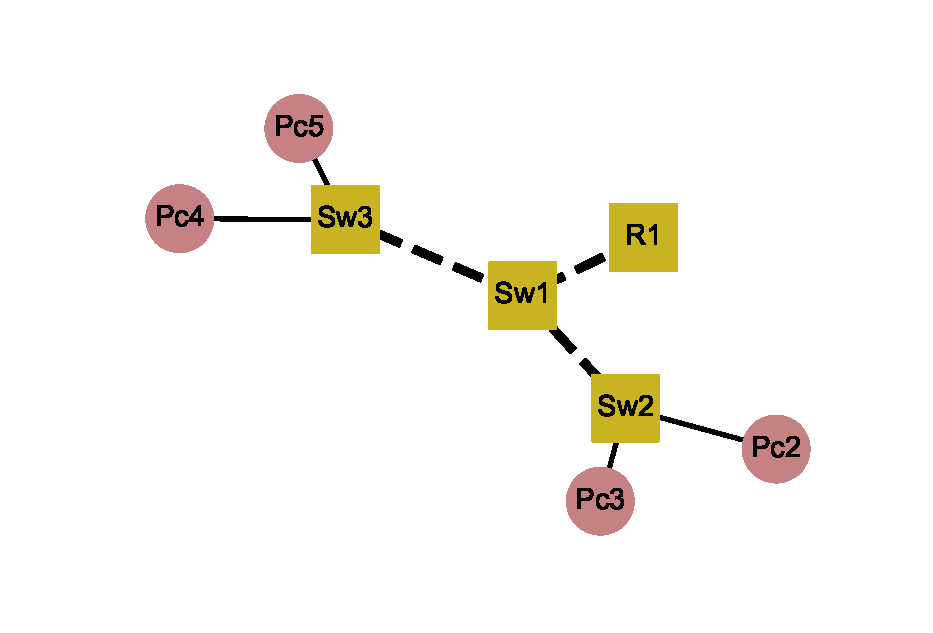
\includegraphics[scale=0.7]{Graf1_spring_layout.eps}
\caption{Grafo simple no dirigido acíclico, donde las lineas discontinuas representan los cables de fibra optica y los lineas continuas los cables UTP.}
\end{center}
\end{figure}

\newpage
\section{Grafo simple no dirigido cíclico}
Un grafo simple no dirigido cíclico puede usarse áreas como geografía. Si se considera un mapa, digamos de Europa: que cada país sea un vértice y conecte dos vértices con una arista si esos países comparten una frontera. Un problema famoso que quedó sin resolver durante más de cien años fue el problema de los cuatro colores. Aproximadamente esto indica que cualquier mapa puede ser coloreado con a lo sumo cuatro colores de tal manera que los países adyacentes no tengan el mismo color. Este problema motivó muchos desarrollos en la teoría de grafos y finalmente se demostró con la ayuda de una computadora en 1976 \cite{rf1}.\linebreak

Otra aplicación es en la representación de redes sociales, una red social se conceptualiza como un grafo, es decir, un conjunto de vértices (o nodos, unidades, puntos) que representan entidades u objetos sociales y un conjunto de líneas que representan una o más relaciones sociales entre ellos \cite {article1}.\linebreak
Por ejemplo, si consideramos un grupo de nueve doctores del núcleo académico de PISIS (Posgrado en Ingeniería de Sistemas) y construimos una red, tomando como vértices a los doctores y la colaboración de ellos en artículos publicados como aristas dará lugar a un grafo simple no dirigido cíclico como se muestra en la figura 2.\linebreak

\textbf{Algorito de diseño}.\linebreak
Después de probar con varios de los algoritmos de diseño existentes, se decide usar para la representación del grafo de la figura 2 el algoritmo \textit{circular layout}, ya que el mismo permite una mejor compresión del grafo del ejemplo en cuestión.


    
\begin{center}
\lstinputlisting[language=Python]{Graf2.py}
\end{center}
\begin{figure}[ht]
\begin{center}
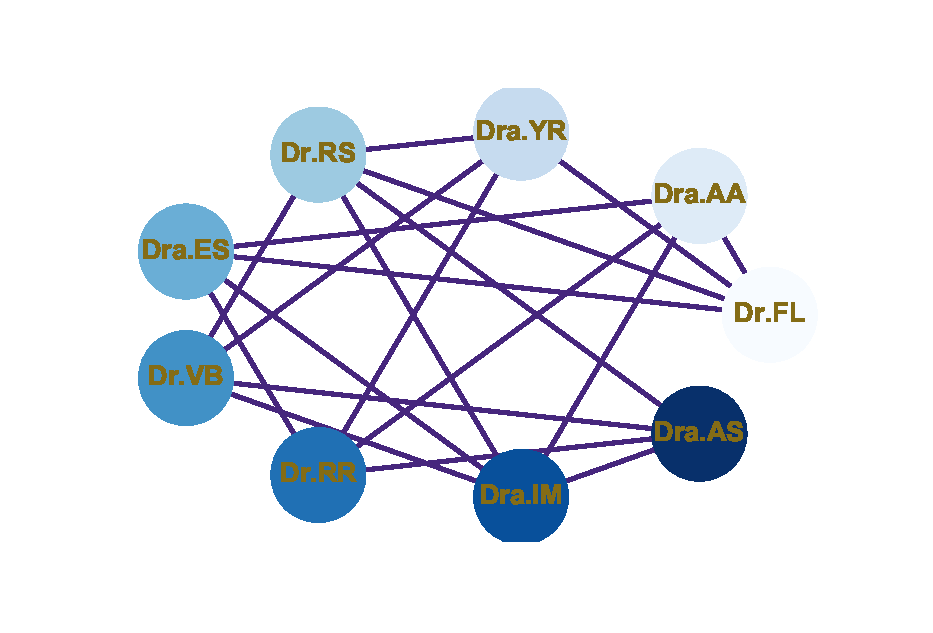
\includegraphics[scale=0.7]{Graf2_circular_layout.eps}\\
\caption{Grafo simple no dirigido cíclico, donde los vértices representa los diferentes doctores y las aristas la colaboración entre ellos.}
\end{center}

\end{figure}

\newpage
\section{Grafo simple no dirigido reflexivo}
Una de las aplicaciones de este tipo de grafo es en la modelación de comportamientos de elementos sociales en la vida real.\linebreak

Por ejemplo, en un estudio sobre el comportamiento sexual de un grupo de adolescentes con edades comprendida entre 15 y 18 años, se representar las relaciones sexuales consentidas (aristas) que existen entre los individuos (vértices) del grupo, así como la satisfacción, para así saber tendencias por edades, posibles esquemas de propagación de enfermedades y promiscuidad entre otros factores del interés de los sexólogos. Este ejemplo se muestra en el grafo de la figura 3.\linebreak

\textbf{Algorito de diseño}.\linebreak
Después de probar con varios de los algoritmos de diseño existentes, se decide usar para la representación del grafo de la figura 3 el algoritmo \textit{kamada kawai layout}, dado que este algoritmo es uno de los más usados para la representación de grafos conexos y no dirigidos, por los resultados de acomodo tan buenos que arroja en estos tipos de grafos.


  
  
\begin{center}
\lstinputlisting[language=Python]{Graf3.py}
\end{center}
\begin{figure}[h]
\begin{center}
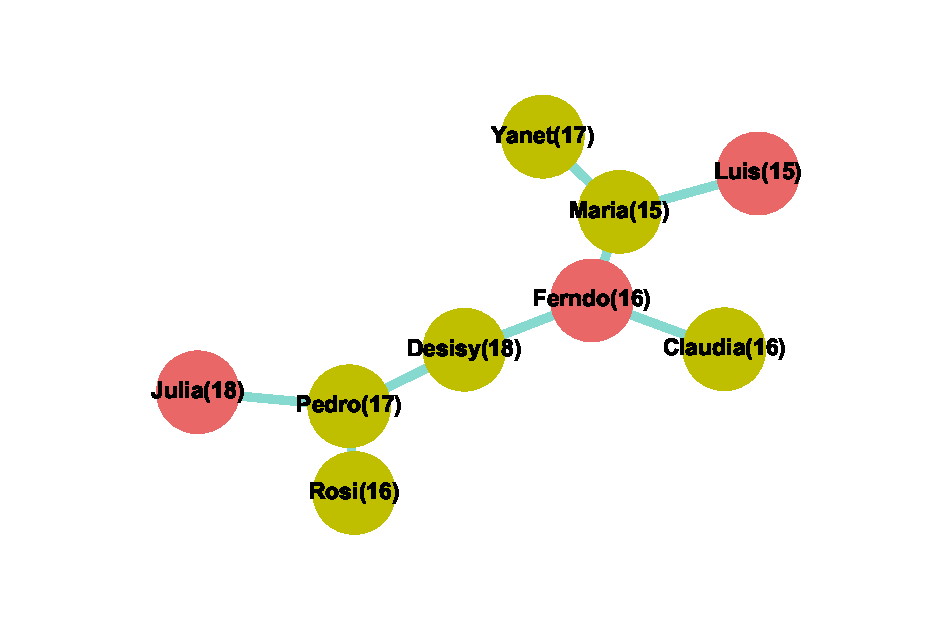
\includegraphics[scale=0.7]{Graf3_kamada_kawai_layout.eps}\\
\caption{Grafo simple no dirigido reflexivo,donde los vértices rojos representan los nodos donde están las aristas reflexivas.}
\end{center}
\end{figure}
\newpage
\section{Grafo simple dirigido acíclico}
Encontraos entre las aplicaciones de los grafos dirigidos o dígrafos acíclico las siguientes: 
\begin{itemize}
\item Una red bayesiana queda especificada formalmente por una dupla $B= (G, O)$, donde $G$ es un grafo dirigido acíclico (GDA) y $O$ es el conjunto de distribuciones de probabilidad. Definimos un grafo como un par $G= (V, E)$, donde $ V $ es un conjunto finito de vértices nodos o variables y $E$ es un subconjunto del producto cartesiano $V \times V $ de pares ordenados de nodos que llamamos enlaces o aristas \cite{gf2}.
\item Los arboles dirigidos son un ejemplo clásico de grafos dirigidos acíclico, estos tienen múltiples en la cotidianidad como pueden ser los arbole genealógicos, los organigramas de una empresa (referido a las jerarquías entre los empleados) y el árbol de directorios de Windows.

\end{itemize}	
En la figura 4 se muestra un ejemplo de red bayesiana (topología de red para el cáncer de pulmón), donde C (cáncer), Con (Contaminación), F (Fumador), D (disnea), Rx (rayos-x) son los vértices y sus relaciones son las aristas.\linebreak 

\textbf{Algorito de diseño}.\linebreak
Después de probar con varios de los algoritmos de diseño existentes, se decide usar para la representación del grafo de la figura 4 el algoritmo \textit{shell layout}, dado que este algoritmo ubica los nodos en círculos concéntricos a un nodo dado, es la mejor opción para representar este ejemplo.



\begin{center}
\lstinputlisting[language=Python]{Graf4.py}
\end{center}

\begin{figure}[h]
\begin{center}
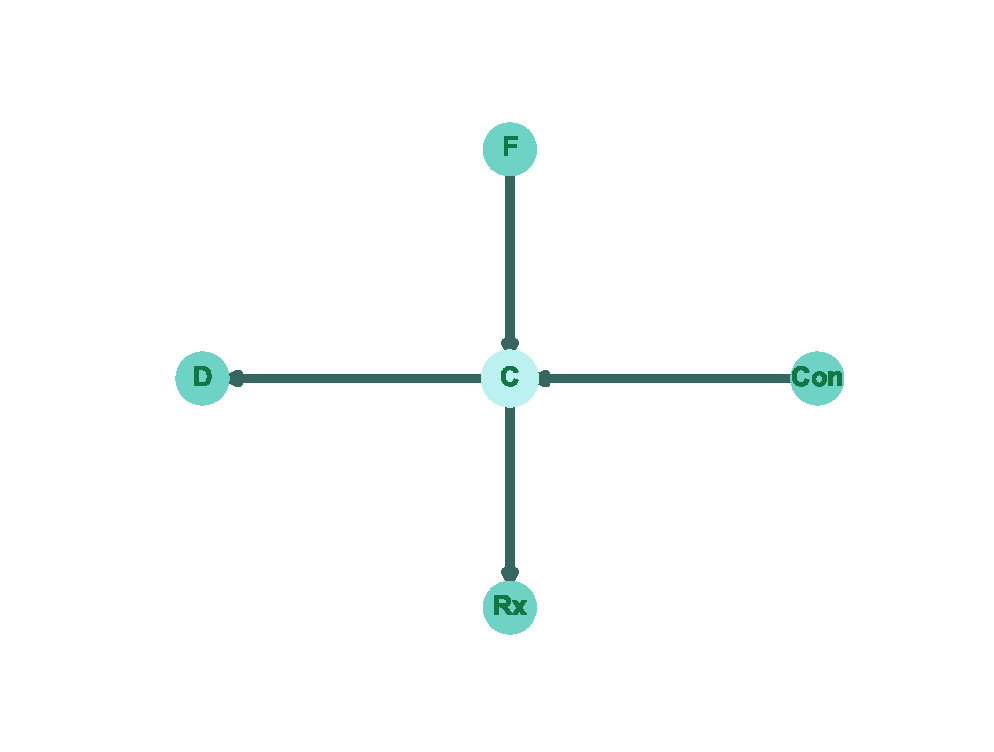
\includegraphics[scale=0.7]{Graf4_shell_layout.eps}\\
\caption{Grafo simple dirigido acíclico.}
\end{center}
\end{figure}
\newpage

\section{Grafo simple dirigido cíclico}
Aplicaciones de los grafos dirigidos cíclicos:
\begin{itemize}
\item En ingeniería eléctrica se utilizan grafos dirigidos cíclicos en el análisis de circuito desde Kirchoff en los años 1850.
\item En redes sociales, otro enfoque de redes sociales en su análisis puede arrojar un grafo dirigido cíclico si te tomamos como vértices a personas y como aristas el sentimiento de amistad de una persona hacia otra, este ejemplo se refleja en el grafo de la figura 5.\linebreak

\textbf{Algorito de diseño}.\linebreak
Después de probar con varios de los algoritmos de diseño existentes, se decide usar para la representación del grafo de la figura 5 el algoritmo \textit{kamada kawai layout}, a pesar de no ser este ejemplo precisamente el más adecuado para este algoritmo fue el de mejor resultado estético.


\end{itemize}
\begin{center}
\lstinputlisting[language=Python]{Graf5.py}
\end{center}

\begin{figure}[h]
\begin{center}
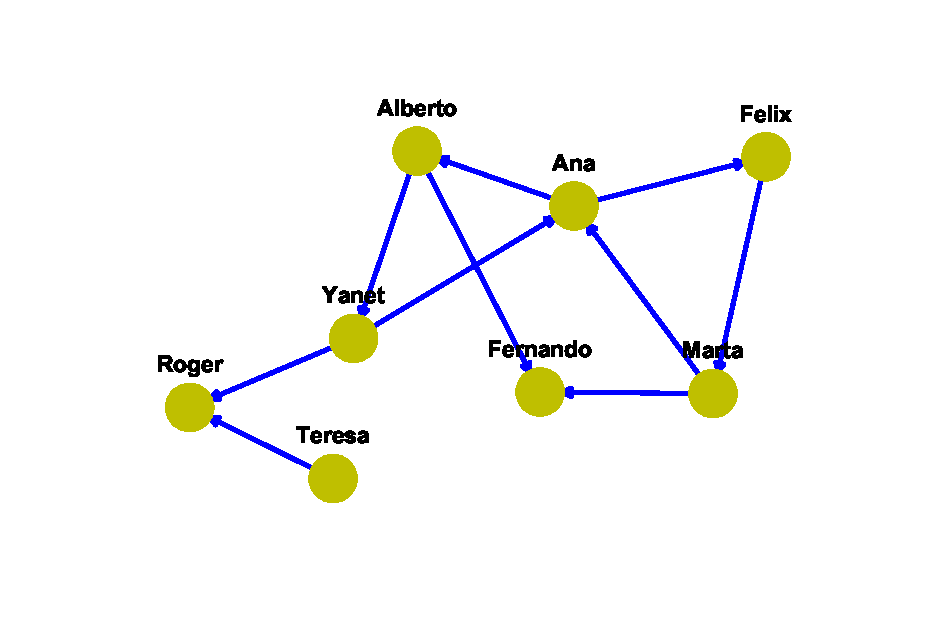
\includegraphics[scale=0.7]{Graf5_kamada_kawai_layout.eps}\\
\caption{Grafo simple dirigido cíclico, donde los vértices representan las personas y las aristas la relación de amistad entre ellas. }
\end{center}
\end{figure}

\newpage

\section{Grafo simple dirigido reflexivo}

Las aplicaciones de estos grafos van desde la representación del funcionamiento de las páginas web, el modelado de una empresa de servicio que brinda el mismo tanto a sus clientes como a ella misma, hasta representar un grafo que modele la comprobación de una red de computadoras.\linebreak

Por ejemplo, suponiendo que se está comprobando la conectividad entre los nodos (equipos) de una red de computadoras, es decir que un nodo puede dar ping a cualquier otro nodo, significa que dicho nodo está conectado con el resto, además se debe asegurar que el mismo nodo pueda recibir un auto ping, si esto no ocurre existe un problema de conectividad. La figura 6 muestra dicho ejemplo.\linebreak

\textbf{Algorito de diseño}.\linebreak
Después de probar con varios de los algoritmos de diseño existentes, se decide usar para la representación del grafo de la figura 6 el algoritmo \textit{random layout}, en este ejemplo se pudo usar este algoritmo por su simpleza ya que con grafos más complejos no es aconsejable el uso del mismo por sus malos resultados estéticamente hablando.


\begin{center}
\lstinputlisting[language=Python]{Graf6.py}
\end{center}
\begin{figure}[ht]
\begin{center}
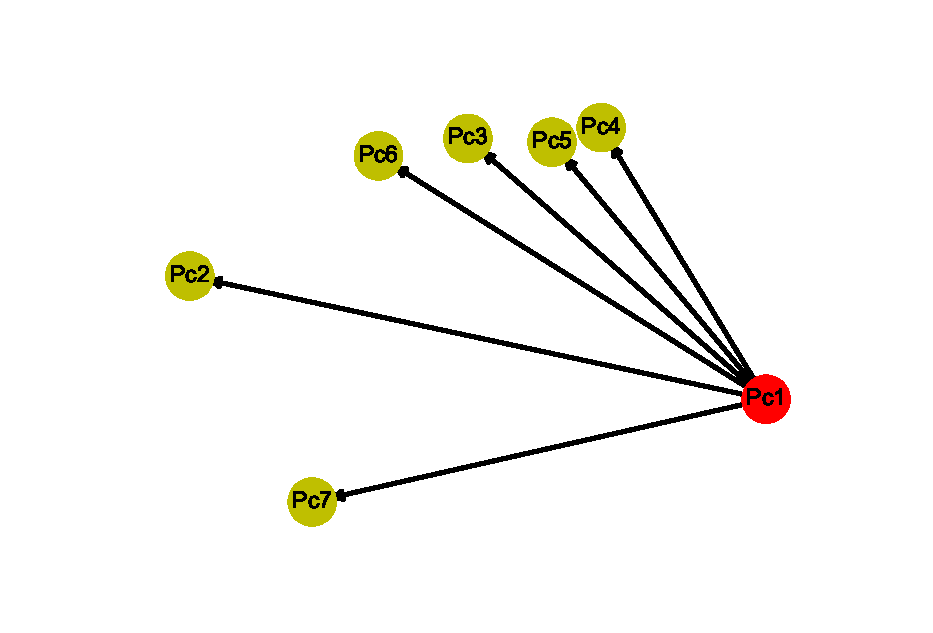
\includegraphics[scale=0.7]{Graf6_random_layout.eps}\\
\caption{Grafo simple dirigido reflexivo, donde el vértice rojo representa la arista reflexiva.}
\end{center}
\end{figure}
\newpage

 \section{Multigrafo no dirigido acíclico}
Una de las aplicaciones de este tipo de grafo es en el tasado de rutas.
Por ejemplo, considerando que se quiere tranzar los diferentes caminos (sin importar el sentido de estos) que comunican a varios Municipios de La Habana en un orden específico (Lisa, Marianao, Playa, Vedado, Habana Vieja, Habana del Este). Tomando como vértices los municipios y como aristas las carreteras que los unen, esto da lugar al grafo que muestra la figura 7.\linebreak

\textbf{Algorito de diseño}.\linebreak
Después de probar con varios de los algoritmos de diseño existentes, se decide usar para la representación del grafo de la figura 7 el algoritmo \textit{spring layout}, este acomoda los nodos con el algoritmo dirigido por fuerza de Fruchterman-Reingold que minimiza la distancia entre los vértices conectados y de mayor peso.
\begin{center}
\lstinputlisting[language=Python]{Graf7.py}
\end{center}
\begin{figure}[h]
\begin{center}
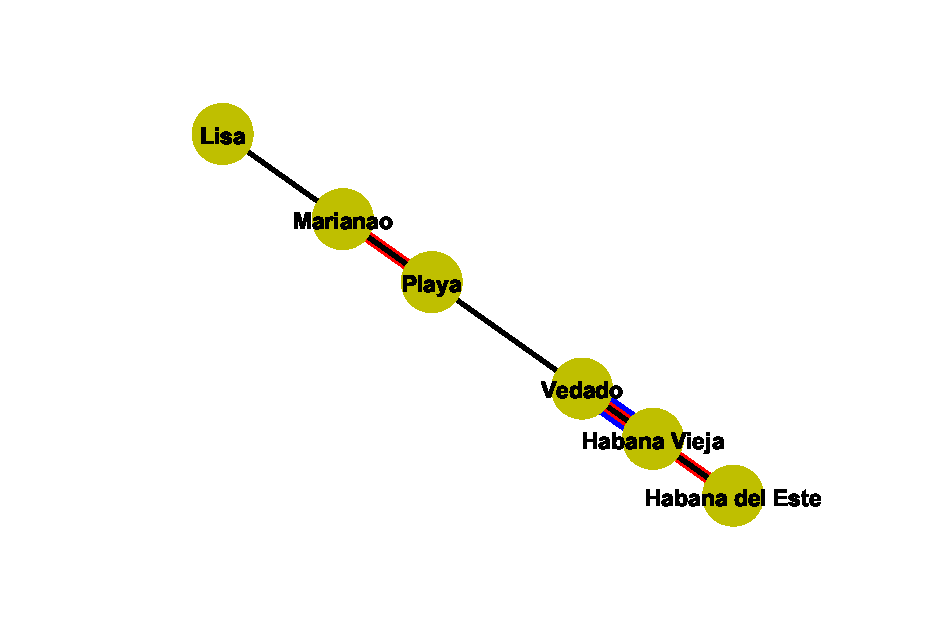
\includegraphics[scale=0.7]{Graf7_spring_layout.eps}\\
\caption{Multigrafo no dirigido acíclico, donde la diferencia de colores de los arcos representan los diferentes caminos.}
\end{center}
\end{figure}
\section{Multigrafo no dirigido cíclico}

Un ejemplo donde podemos utilizar este tipo de grafos es: se quiere representar cuantas llamadas (aristas)se realizaron entre un grupo de personas (vértices), donde nos importa saber la duración de cada llamada durante un día determinado. Este grafo se ve representado en la figura 8.\linebreak

\textbf{Algorito de diseño}.\linebreak
Después de probar con varios de los algoritmos de diseño existentes, se decide usar para la representación del grafo de la figura 8 el algoritmo \textit{spectral layout}, dando buenos resultados estetico.


\begin{center}
\lstinputlisting[language=Python]{Graf8.py}
\end{center}
\begin{figure}[h]
\begin{center}
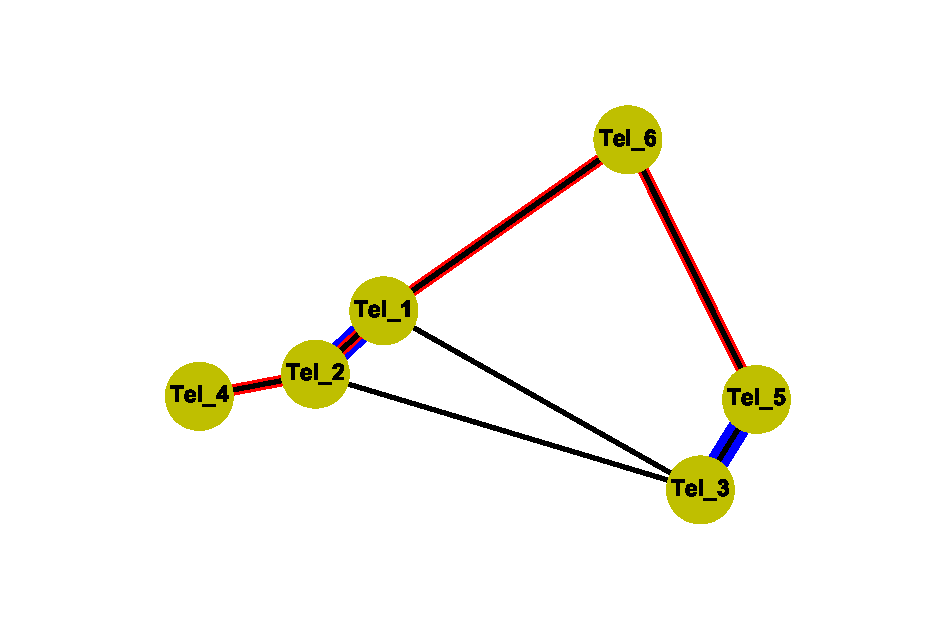
\includegraphics[scale=0.7]{Graf8_spectral_layout.eps}\\
\caption{Multigrafo no dirigido cíclico, donde las aristas de diferentes colores representan la existencia de las llamadas con distinta duración.}
\end{center}
\end{figure}
\section{Multigrafo no dirigido reflexivo}
Partiendo del ejemplo de la sección 3 se pretende construir un grafo más informativo a la hora de su análisis, por lo que se le agrega como arista (el hecho que las relaciones sexuales mantenidas fueran dentro de una relación formal). Este grafo se muestra en la figura 9.\linebreak

\textbf{Algorito de diseño}.\linebreak
Después de probar con varios de los algoritmos de diseño existentes, se decide usar para la representación del grafo de la figura 9 el algoritmo \textit{circular layout}, ya que el mismo permite una mejor compresión de este ejemplo mediante la ubicación circular de los nodos.

\begin{center}
\lstinputlisting[language=Python]{Graf9.py}
\end{center}
\begin{figure}[h]
\begin{center}
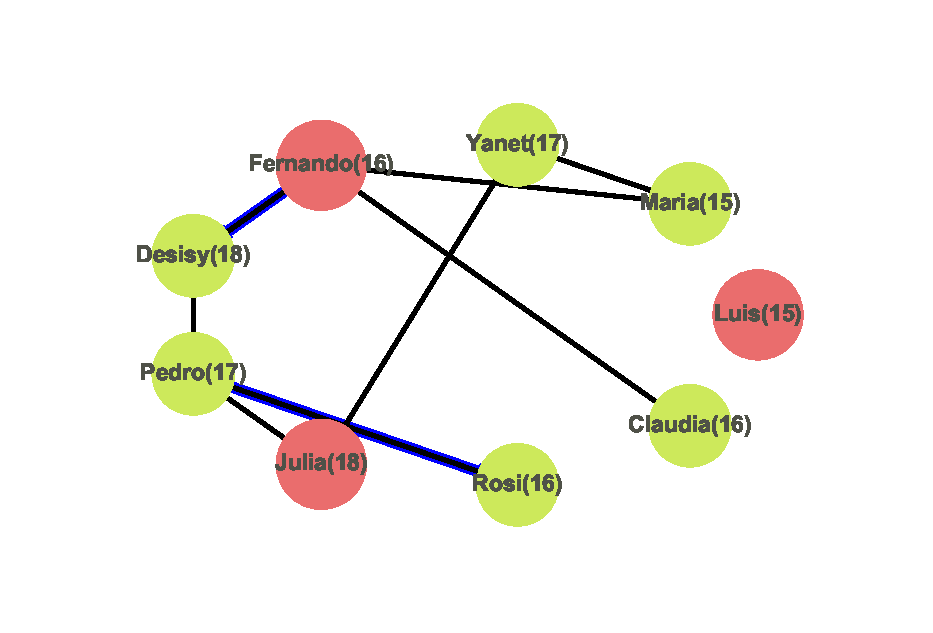
\includegraphics[scale=0.7]{Graf9_circular_layout.eps}\\
\caption{Multigrafo no dirigido reflexivo, donde las aristas de diferentes colores representan la existencia de una relación formal entre los individuos y los vértices de color rojo representa los vértices con aristas reflexivas.}
\end{center}
\end{figure}
\section{Multigrafo dirigido acíclico}
Considerando que se quiere trazar las diferentes rutas (teniendo en cuenta el sentido de los mimas) que llevan de una provincia a otra en Cuba (Pinar del Río, Artemisa, La Habana, Mayabeque, Matanza, Cienfuegos, Villa Clara). Tomando como vértices las provincias y como aristas las carreteras que las unen, como muestra la figura 10.\linebreak

\textbf{Algorito de diseño}.\linebreak
Después de probar con varios de los algoritmos de diseño existentes, se decide usar para la representación del grafo de la figura 10 el algoritmo \textit{spectral layout}, ya que el mismo logro un buen resultado en la ubicación de los nodos facilitando la compresión del grafo.
\begin{center}
\lstinputlisting[language=Python]{Graf10.py}
\end{center}
\begin{figure}[h]
\begin{center}
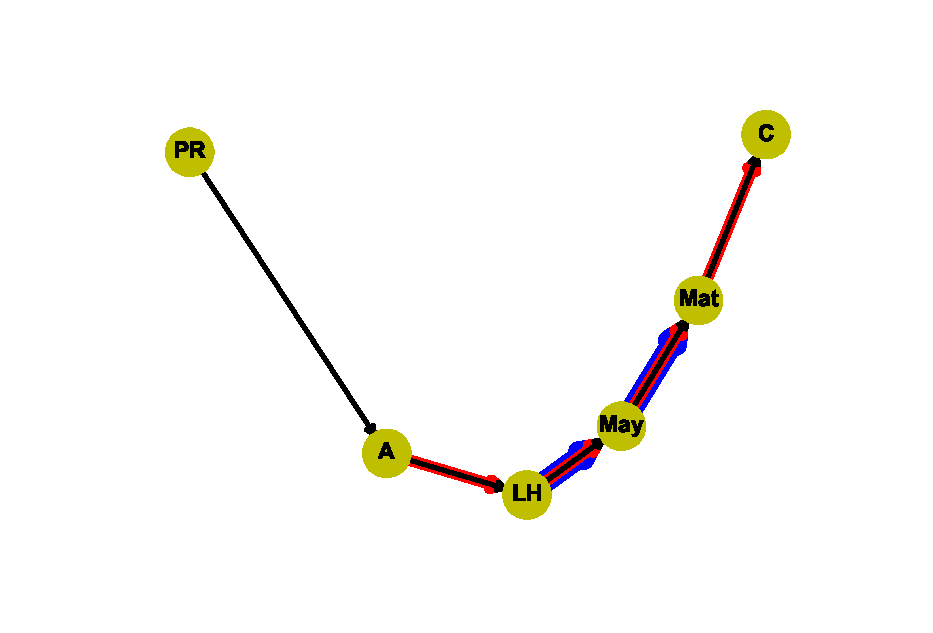
\includegraphics[scale=0.7]{Graf10_spectral_layout.eps}\\
\caption{Multigrafo dirigido acíclico, donde las aristas de diferentes colores representan las existencia de mas de una ruta entre las diferente provincias.}
\end{center}
\end{figure}
\newpage
\section{Mltigrafo dirigido cíclico}
“En el caso particular de que las redes reflejen una realidad social, los nodos pueden representar personas o entidades relacionadas con sus contextos, y las conexiones representarán relaciones sociales existentes entre ellos (amistad, parentesco, membresía, afinidad, etc.). A pesar de que intuitivamente las redes sociales se asemejan a los grafos matemáticos, es más habitual que en ellas se trabaje con distintos tipos de relaciones"\cite{gf3} por lo que es necesario la utilización de multígrafos, que es la herramienta que contempla más de una relación entre dos nodos, con esto ganamos mayor riqueza en los datos a analizar.\linebreak 
Por ejemplo, tenemos un grupo de personas que laboran en un departamento de Informática y se hace una encuesta donde se les pide que marque cuales de tres sentimientos (respeto, afinidad, rechazo) sienten por sus compañeros de trabajo, como muestra la figura 11.\linebreak

\textbf{Algorito de diseño}.\linebreak
Después de probar con varios de los algoritmos de diseño existentes, se decide usar para la representación del grafo de la figura 11 el algoritmo \textit{kamada kawai layout}, ya que el mismo logro un buen resultado estético.


\begin{center}
\lstinputlisting[language=Python]{Graf11.py}
\end{center}
\begin{figure}[h]
\begin{center}
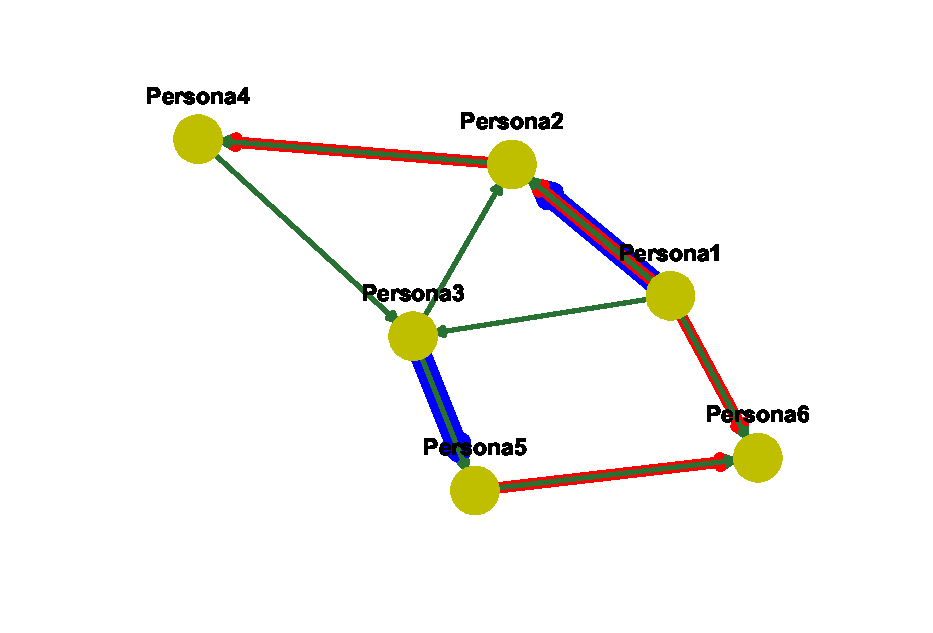
\includegraphics[scale=0.7]{Graf11_kamada_kawai_layout.eps}\\
\caption{Multigrafo dirigido cíclico, donde las aristas de diferentes colores representan las existencia de más de una opinión sobre sus compañeros.}
\end{center}
\end{figure}
\newpage
\section{Multigrafo dirigido reflexivo}
Una de las aplicaciones de estos grafos es en el modelado del funcionamiento de una máquina de estados.
Por ejemplo, se desea modelar un grafo que represente el funcionamiento de una máquina muy sencilla de golosinas, que responde a las siguientes reglas:

\begin{itemize}
\item[1] Cada golosina vale \$ 0.25.
\item[2] La máquina acepta sólo monedas de  \$ 0.10 y de \$ 0.05.
\item[3] La máquina NO da vuelto.
\end{itemize}
Para modelar el grafo, debemos considerar distintos “estados de dinero ingresado”, y como se va pasando de uno a otro. Por ejemplo, si en un momento tenemos ingresados 5 centavos, y agregamos 5 centavos más, pasamos a otro estado, que es el mismo que si hubiésemos ingresado 10 centavos al principio. Llamemos A, B, C, D, E y F a los estados que representan 0, 5, 10, 15, 20, 25 centavos ingresados respectivamente. Las transiciones de un estado a otro se harán por ingreso de 5 o 10 centavos, o al presionar el botón para obtener los caramelos (G). Como se muestra en la figura 12. \linebreak

\textbf{Algorito de diseño}.\linebreak
Después de probar con varios de los algoritmos de diseño existentes, se decide usar para la representación del grafo de la figura 12 el algoritmo \textit{spectral layout}, ya que este algoritmo mostro el mejor de los resultados a la hora de representar este ejemplo.
\begin{center}
\lstinputlisting[language=Python]{Graf12.py}
\end{center}
\begin{figure}[h]
\begin{center}
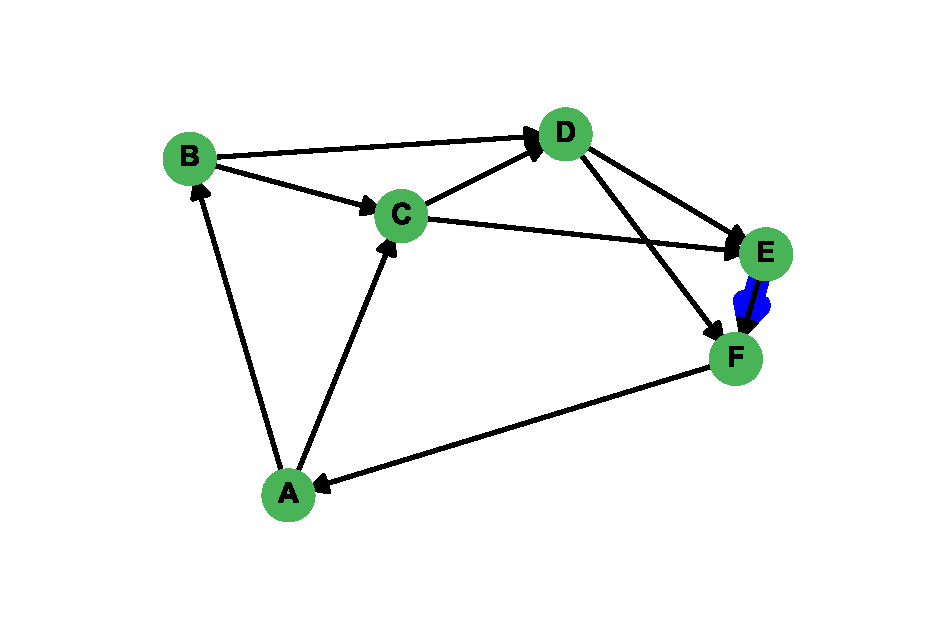
\includegraphics[scale=0.7]{Graf12_spectral_layout.eps}\\
\caption{Multigrafo dirigido reflexivo, donde las aristas de diferentes colores representan las existencia de mas de una forma de pasar de un estado a otro.}
\end{center}
\end{figure}
\newpage

\bibliography{tarea2}
\bibliographystyle{plain}
\end{document}
